\documentclass[tikz,border=10pt]{standalone}
\usepackage{amsmath,amssymb}
\usepackage{tikz}
\usetikzlibrary{arrows.meta,calc,positioning}

\definecolor{navy}{HTML}{1B365D}
\definecolor{steelblue}{HTML}{2471A3}
\definecolor{softblue}{HTML}{D4E6F1}
\definecolor{teal}{HTML}{0E6251}
\definecolor{softteal}{HTML}{D1F2EB}
\definecolor{amber}{HTML}{B9770E}
\definecolor{softamber}{HTML}{FCF3CF}
\definecolor{crimson}{HTML}{922B21}
\definecolor{softred}{HTML}{FADBD8}
\definecolor{slate}{HTML}{566573}

\begin{document}
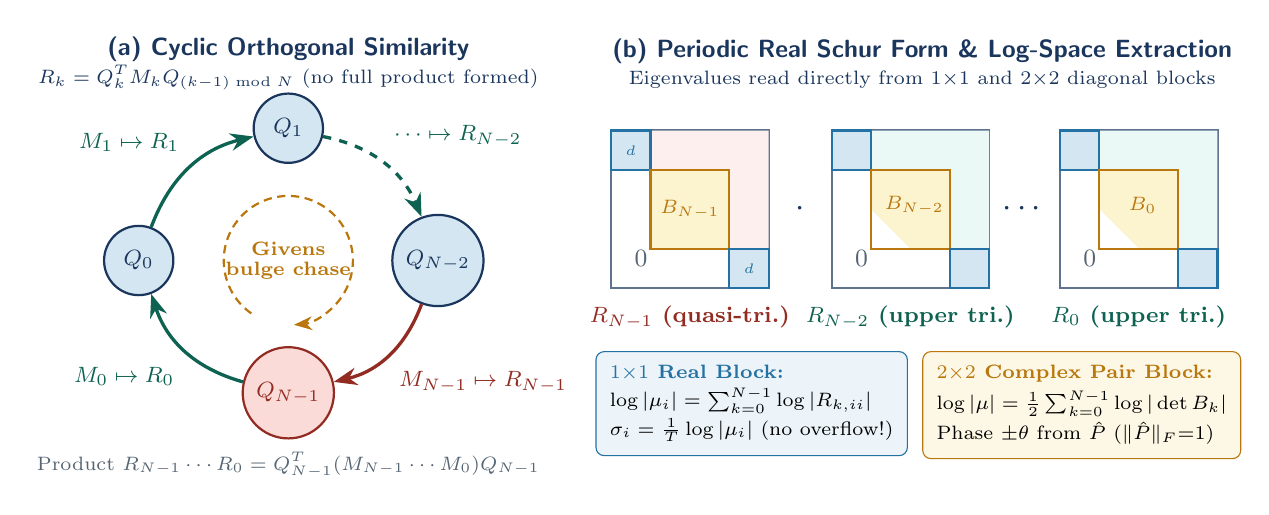
\begin{tikzpicture}[
    >=Stealth,
    font=\sffamily\footnotesize,
]

% ========================
% LEFT PANEL: Cyclic Similarity Chain & Givens Bulge Propagation
% ========================
\begin{scope}[shift={(0,0)}]
    \node[font=\sffamily\bfseries\small, navy, align=center] at (2.8, 4.95)
        {(a) Cyclic Orthogonal Similarity\\[-1pt]\normalfont\scriptsize $R_k = Q_k^T M_k Q_{(k-1)\bmod N}$ (no full product formed)};

    % Draw 4 state nodes in a circle (centered at (2.8, 2.45))
    \coordinate (C) at (2.8, 2.45);
    \node[circle, draw=navy, fill=softblue, thick, minimum size=0.88cm, font=\sffamily\footnotesize\bfseries, text=navy]
        (q0) at ($(C) + (180:1.90)$) {$Q_0$};
    \node[circle, draw=navy, fill=softblue, thick, minimum size=0.88cm, font=\sffamily\footnotesize\bfseries, text=navy]
        (q1) at ($(C) + (90:1.68)$) {$Q_1$};
    \node[circle, draw=navy, fill=softblue, thick, minimum size=0.88cm, font=\sffamily\footnotesize\bfseries, text=navy]
        (q2) at ($(C) + (0:1.90)$) {$Q_{N-2}$};
    \node[circle, draw=crimson, fill=softred, thick, minimum size=0.88cm, font=\sffamily\footnotesize\bfseries, text=crimson]
        (q3) at ($(C) + (270:1.68)$) {$Q_{N-1}$};

    % Curved arrows between orthogonal bases representing M_k -> R_k
    \draw[->, very thick, teal] (q0) to[bend left=28]
        node[above left=2pt and 0pt, teal, font=\footnotesize\bfseries] {$M_1 \mapsto R_1$} (q1);
    \draw[->, very thick, teal, dashed] (q1) to[bend left=28]
        node[above right=2pt and 0pt, teal, font=\footnotesize\bfseries] {$\cdots \mapsto R_{N-2}$} (q2);
    \draw[->, very thick, crimson] (q2) to[bend left=28]
        node[below right=2pt and 0pt, crimson, font=\footnotesize\bfseries] {$M_{N-1} \mapsto R_{N-1}$} (q3);
    \draw[->, very thick, teal] (q3) to[bend left=28]
        node[below left=2pt and 0pt, teal, font=\footnotesize\bfseries] {$M_0 \mapsto R_0$} (q0);

    % Center annotation: Givens bulge chasing loop
    \draw[->, thick, amber, dash pattern=on 3pt off 2pt]
        ($(C) + (235:0.82)$) arc[start angle=235, end angle=-85, radius=0.82];
    \node[amber, font=\scriptsize\bfseries, align=center] at (C)
        {Givens\\[-1pt]bulge chase};

    \node[slate, font=\scriptsize, align=center] at (2.8, -0.15)
        {Product $R_{N-1} \cdots R_0 = Q_{N-1}^T (M_{N-1} \cdots M_0) Q_{N-1}$};
\end{scope}

% ========================
% RIGHT PANEL: Periodic Real Schur Factors & Log-Space Eigenvalue Extraction
% ========================
\begin{scope}[shift={(6.7, 0.25)}]
    \node[font=\sffamily\bfseries\small, navy, align=center] at (4.15, 4.70)
        {(b) Periodic Real Schur Form \& Log-Space Extraction\\[-1pt]\normalfont\scriptsize Eigenvalues read directly from $1{\times}1$ and $2{\times}2$ diagonal blocks};

    % Draw R_{N-1} (quasi-upper-triangular with a 1x1 block and a 2x2 block)
    \begin{scope}[shift={(0.2, 1.85)}]
        \draw[thick, navy!70] (0,0) rectangle (2.0, 2.0);
        \fill[softred!45] (0, 2.0) -- (2.0, 2.0) -- (2.0, 0.0) -- cycle;
        \fill[softblue, draw=steelblue, thick] (0.0, 1.5) rectangle (0.5, 2.0);
        \node[steelblue, font=\tiny\bfseries] at (0.25, 1.75) {$d$};
        \fill[softamber, draw=amber, thick] (0.5, 0.5) rectangle (1.5, 1.5);
        \node[amber, font=\scriptsize\bfseries] at (1.0, 1.0) {$B_{N-1}$};
        \fill[softblue, draw=steelblue, thick] (1.5, 0.0) rectangle (2.0, 0.5);
        \node[steelblue, font=\tiny\bfseries] at (1.75, 0.25) {$d$};
        \node[slate, font=\small] at (0.38, 0.38) {$0$};
        \node[crimson, font=\footnotesize\bfseries, below=3pt] at (1.0, 0) {$R_{N-1}$ (quasi-tri.)};
    \end{scope}

    \node[navy, font=\large] at (2.60, 2.85) {$\cdot$};

    % Draw R_{N-2} (strictly upper triangular)
    \begin{scope}[shift={(3.0, 1.85)}]
        \draw[thick, navy!70] (0,0) rectangle (2.0, 2.0);
        \fill[softteal!45] (0, 2.0) -- (2.0, 2.0) -- (2.0, 0.0) -- cycle;
        \fill[softblue, draw=steelblue, thick] (0.0, 1.5) rectangle (0.5, 2.0);
        \fill[softamber, draw=amber, thick] (0.5, 0.5) rectangle (1.5, 1.5);
        \fill[white] (0.5, 0.5) -- (1.0, 0.5) -- (0.5, 1.0) -- cycle;
        \draw[amber, thick] (0.5, 0.5) rectangle (1.5, 1.5);
        \node[amber, font=\scriptsize\bfseries] at (1.05, 1.05) {$B_{N-2}$};
        \fill[softblue, draw=steelblue, thick] (1.5, 0.0) rectangle (2.0, 0.5);
        \node[slate, font=\small] at (0.38, 0.38) {$0$};
        \node[teal, font=\footnotesize\bfseries, below=3pt] at (1.0, 0) {$R_{N-2}$ (upper tri.)};
    \end{scope}

    \node[navy, font=\large] at (5.45, 2.85) {$\cdots$};

    % Draw R_0 (strictly upper triangular)
    \begin{scope}[shift={(5.9, 1.85)}]
        \draw[thick, navy!70] (0,0) rectangle (2.0, 2.0);
        \fill[softteal!45] (0, 2.0) -- (2.0, 2.0) -- (2.0, 0.0) -- cycle;
        \fill[softblue, draw=steelblue, thick] (0.0, 1.5) rectangle (0.5, 2.0);
        \fill[softamber, draw=amber, thick] (0.5, 0.5) rectangle (1.5, 1.5);
        \fill[white] (0.5, 0.5) -- (1.0, 0.5) -- (0.5, 1.0) -- cycle;
        \draw[amber, thick] (0.5, 0.5) rectangle (1.5, 1.5);
        \node[amber, font=\scriptsize\bfseries] at (1.05, 1.05) {$B_0$};
        \fill[softblue, draw=steelblue, thick] (1.5, 0.0) rectangle (2.0, 0.5);
        \node[slate, font=\small] at (0.38, 0.38) {$0$};
        \node[teal, font=\footnotesize\bfseries, below=3pt] at (1.0, 0) {$R_0$ (upper tri.)};
    \end{scope}

    % Formula summary boxes below (cleanly separated!)
    \node[draw=steelblue, fill=softblue!45, rounded corners=3pt, align=left,
          font=\scriptsize, anchor=north west, inner sep=5pt] at (0.0, 1.05) {%
        \textbf{\color{steelblue}$1{\times}1$ Real Block:}\\[2pt]
        $\log|\mu_i| = \sum_{k=0}^{N-1} \log |R_{k,ii}|$\\[1pt]
        $\sigma_i = \frac{1}{T}\log|\mu_i|$ (no overflow!)%
    };

    \node[draw=amber, fill=softamber!55, rounded corners=3pt, align=left,
          font=\scriptsize, anchor=north west, inner sep=5pt] at (4.15, 1.05) {%
        \textbf{\color{amber}$2{\times}2$ Complex Pair Block:}\\[2pt]
        $\log|\mu| = \frac{1}{2}\sum_{k=0}^{N-1} \log |\det B_k|$\\[1pt]
        Phase $\pm\theta$ from $\hat{P}$ ($\|\hat{P}\|_F{=}1$)%
    };
\end{scope}

\end{tikzpicture}
\end{document}
